\chapter{Introduzione e concetti generali di Software Testing}

\section{Qualità, Verifica e Validazione}

Nei sistemi software esiste spesso una discrepanza tra ciò che il cliente desidera, ciò che viene progettato, ciò che viene implementato e ciò che è realmente necessario. Questa distanza rende necessario introdurre attività sistematiche di garanzia della qualità.


Citando Boehm, le attività di Verifica e Validazione rispondono a due domande diverse:

\begin{itemize}
    \item \textbf{Verifica}: \emph{Are we building the product right?}
    Controlla se il prodotto è conforme alle specifiche tecniche.

    \item \textbf{Validazione}: \emph{Are we building the right product?}
    Controlla se il prodotto soddisfa le attese del committente o dell'utente.
\end{itemize}

L'obiettivo delle attività di V\&V è rassicurare l'utilizzatore che il sistema sia adatto allo scopo. Il livello di fiducia fornito non è assoluto, ma dipende dal contesto.

\begin{notaprof}
Il livello di confidenza richiesto varia in base alla funzione del software. Un gestionale per documenti richiede garanzie diverse rispetto a un sistema safety-critical che può prendere decisioni vitali.
\end{notaprof}

\section{Modello formale \(P, S, D, C\)}

Per formalizzare il problema della verifica si considerano quattro elementi:

\begin{itemize}
    \item \textbf{\(S\)}: specifica, cioè descrizione del comportamento atteso;
    \item \textbf{\(D\)}: dominio degli input;
    \item \textbf{\(C\)}: codominio degli output;
    \item \textbf{\(P\)}: programma, cioè funzione che mappa elementi di \(D\) in \(C\).
\end{itemize}

Un programma \(P\) soddisfa la specifica \(S\) se e solo se, per ogni input \(d \in D\), vale:

\[
P(d) = S(d)
\]

\begin{figure}[H]
    \centering
    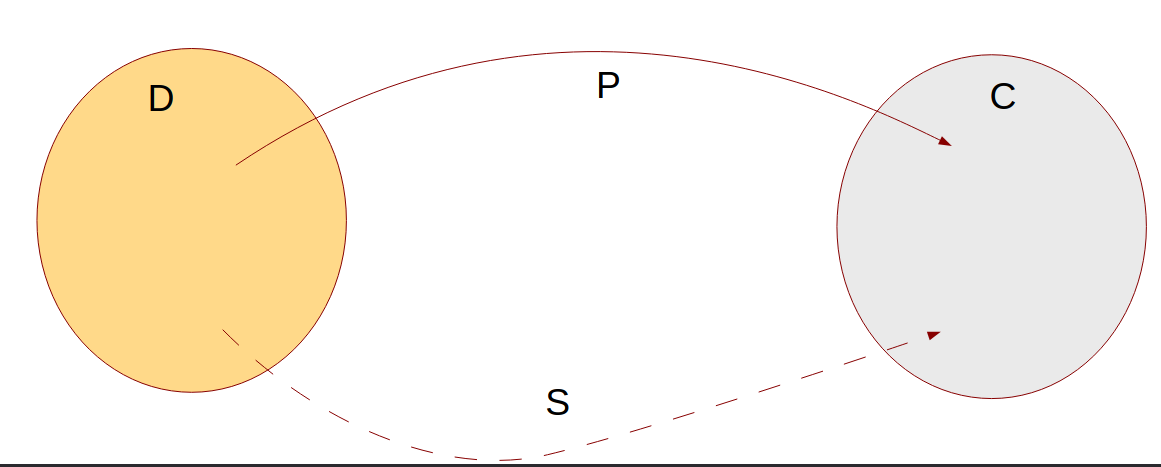
\includegraphics[width=0.65\textwidth]{img/DeAngelis/02_GeneralConcepts/dominio.png}
    \caption{Rappresentazione del dominio \(D\), del codominio \(C\), del programma \(P\) e della specifica \(S\). Il programma è corretto rispetto alla specifica quando, per ogni input del dominio, il comportamento prodotto da \(P\) coincide con quello atteso da \(S\).}
    \label{fig:modello-psdc}
\end{figure}


\section{Verifica formale, testing e debugging}

Esistono approcci diversi per obiettivi diversi.

La \textbf{verifica formale} mira a dimostrare matematicamente che il programma \(P\) soddisfa la specifica \(S\) su ogni possibile input.

\begin{notaprof}
La verifica formale richiede competenze specialistiche, ad esempio in logica, grafi o algebra. Spesso opera su modelli astratti del sistema e non direttamente sul codice eseguito in produzione.
\end{notaprof}

Il \textbf{software testing} mira invece a cercare differenze tra \(P\) e \(S\) tramite esperimenti su un sottoinsieme di input.

Il \textbf{debugging} è l'attività che segue l'osservazione di una difformità: serve a individuare la causa del problema e a rimuoverla.

\begin{notaesame}
Testing e debugging non sono la stessa cosa. Il testing cerca di evidenziare una failure, cioè di mostrare che il programma si comporta diversamente dalla specifica. Il debugging interviene dopo, per capire la causa e correggere il difetto.
\end{notaesame}

\section{Failure, Fault, Error}

La definizione banale ``corretto = senza errori'' non è sufficiente. È necessario distinguere tra tre concetti:

\begin{itemize}
    \item \textbf{Failure} o \textbf{malfunzionamento}: comportamento non corretto e osservabile dall'esterno;
    \item \textbf{Fault}, \textbf{bug} o \textbf{difetto}: problema presente nel codice o nel modello;
    \item \textbf{Error} o \textbf{errore}: causa originaria del fault, spesso dovuta a un errore umano.
\end{itemize}

La relazione causale è:

\[
\text{Error} \rightarrow \text{Fault} \rightarrow \text{Failure}
\]

Un errore umano introduce un fault nel codice; il fault, se attivato in certe condizioni, può manifestarsi come failure.

\begin{figure}[H]
    \centering
    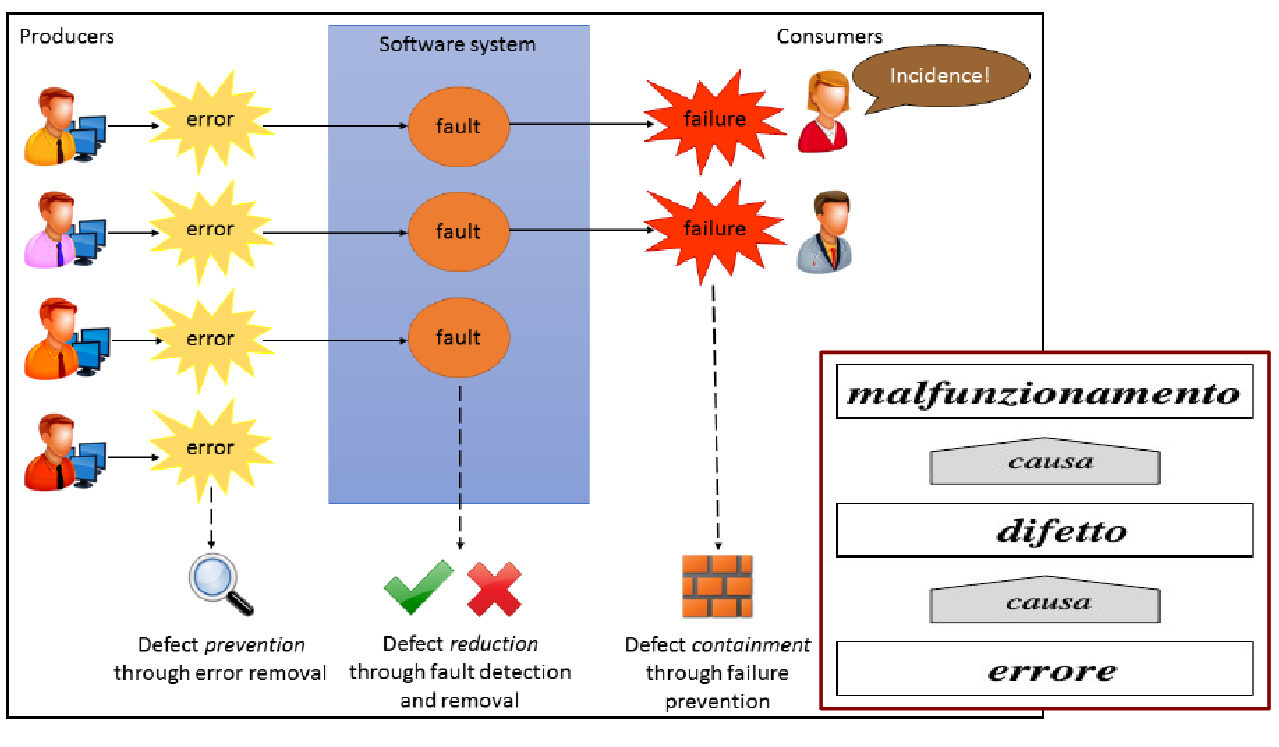
\includegraphics[width=0.9\textwidth]{img/DeAngelis/02_GeneralConcepts/ffe.png}
    \caption{Relazione tra \emph{error}, \emph{fault} e \emph{failure}: l'errore umano introduce un difetto nel sistema software, che può manifestarsi all'utente come malfunzionamento osservabile. La figura evidenzia anche tre strategie di intervento: prevenzione degli errori, rilevazione e rimozione dei fault, e contenimento delle failure.}
    \label{fig:error-fault-failure}
\end{figure}

\subsection{Esempio \texttt{makeItDouble}}

Si consideri la funzione:

\begin{verbatim}
int makeItDouble(int param) {
    int result;
    result = param * param;
    return(result);
}
\end{verbatim}

La chiamata \texttt{makeItDouble(3)} restituisce \(9\), ma se la specifica richiede il raddoppio del parametro, il risultato atteso sarebbe \(6\).

In questo caso:

\begin{itemize}
    \item \(9\) è la \textbf{failure}, cioè il risultato osservabile errato;
    \item \texttt{param * param} è il \textbf{fault}, cioè il difetto nel codice;
    \item l'\textbf{error} può essere un typo oppure un errore di interpretazione tra ``double'' e ``power''.
\end{itemize}


\section{Software Testing}

Il \textbf{software testing} consiste nell'esecuzione di esperimenti in un ambiente controllato, con lo scopo di acquisire sufficiente fiducia sul funzionamento del sistema.

Il testing riguarda tipicamente aspetti funzionali, ma può riguardare anche caratteristiche extra-funzionali.

I principali vantaggi sono:

\begin{itemize}
    \item verificare se il sistema risponde alle esigenze per cui è stato creato;
    \item rendere osservabili eventuali malfunzionamenti.
\end{itemize}

Il limite fondamentale è che il testing non può dimostrare l'assenza di difetti.

\begin{notaesame}
Secondo Dijkstra, il software testing può dimostrare la presenza di guasti, ma non la loro assenza. Se un test fallisce, sappiamo che esiste un problema; se tutti i test passano, sappiamo solo che non abbiamo trovato problemi nei casi testati.
\end{notaesame}


\section{Esempio \texttt{myBuggyFact} e dominio di input}

La specifica dell'esempio richiede il calcolo del fattoriale su tutti gli interi, interpretando il fattoriale di un numero negativo come il fattoriale del suo opposto.

La funzione mostrata è:

\begin{verbatim}
int myBuggyFact(int p){
    int result = abs(p);
    if (result > 1){
        int next = result - 1;
        result = result * myBuggyFact(next);
    }
    return result;
}
\end{verbatim}

Il dominio degli input è molto ampio: per un intero a 32 bit ci sono \(2^{32}\) possibili valori. L'esplorazione esaustiva è quindi impraticabile.

\begin{notaslide}
Le slide usano la metafora dell'ago nel pagliaio per rappresentare la difficoltà di trovare l'input che manifesta il difetto all'interno di un dominio enorme.
\end{notaslide}

Per questo motivo occorre selezionare in modo intelligente solo alcune parti del dominio, ad esempio usando classi di equivalenza.

\section{Domande fondamentali del testing}

La progettazione dei test richiede di rispondere ad alcune domande fondamentali.

\subsection{Quali e quanti input selezionare?}

Poiché non è possibile testare tutto il dominio, bisogna scegliere valori rappresentativi. Una strategia consiste nel partizionare il dominio in classi di equivalenza rispetto a un certo obiettivo di test.

\subsection{Quando smettere di testare?}

Servono criteri di copertura e valori minimi di accettazione. Tra i criteri possibili ci sono:

\begin{itemize}
    \item copertura degli statement;
    \item copertura degli archi;
    \item copertura delle condizioni;
    \item copertura dei flussi;
    \item copertura delle funzionalità.
\end{itemize}

\subsection{Come sapere se il risultato è corretto?}

Questo è l'\textbf{oracle problem}: per stabilire se un test passa o fallisce, bisogna conoscere l'output atteso.

\begin{notaprof}
L'oracolo può derivare da specifiche, dati storici, tabelle note o sistemi equivalenti già in esecuzione. Tuttavia, in generale, sapere automaticamente quale sia l'output corretto non è sempre banale.
\end{notaprof}

\section{Testing come campionamento}

In generale, il dominio \(D\) è molto grande e l'esplorazione esaustiva non è praticabile. Inoltre, solo una piccola parte del dominio può causare errori.

Di conseguenza, il testing può essere visto come l'esecuzione del programma su un \textbf{campione} di dati di input.

\[
\text{Testing} = \text{eseguire un programma su un campione di input}
\]

Questo approccio permette di aumentare la confidenza nel sistema, ma non fornisce certezza assoluta di correttezza.

\section{Correttezza vs Reliability}

La \textbf{correttezza} di un programma indica la completa aderenza alle specifiche per ogni elemento del dominio di input. Può essere asserita tramite prove formali, oppure richiederebbe un testing esaustivo, impraticabile nella maggior parte dei casi.

La \textbf{reliability}, invece, è un attributo statistico del sistema. Indica la probabilità che un'interazione con il programma termini con successo, assumendo un certo profilo di utilizzo.

La formula è:

\[
Reliability = 1 - PFD
\]

dove \(PFD\) è la \emph{Probability of Failure on Demand}.

\begin{notaesame}
Un sistema può avere alta reliability senza essere matematicamente corretto. La reliability dipende da come il sistema viene usato, mentre la correttezza richiede aderenza alle specifiche su tutto il dominio.
\end{notaesame}

\section{Operational Profile}

L'\textbf{operational profile} è una descrizione numerica di come il sistema viene effettivamente utilizzato.

Può variare in funzione delle tipologie di utenti e può essere:

\begin{itemize}
    \item \textbf{stimato}, tramite requisiti, specifiche e aspettative di sviluppatori o stakeholder;
    \item \textbf{misurato}, tramite monitoraggio delle richieste al sistema, log e report.
\end{itemize}

\begin{notaprof}
La stessa funzione può avere reliability diverse in base al profilo d'uso. Se gli utenti usano spesso input che attivano il fault, la reliability sarà bassa; se quegli input sono rari, la reliability percepita può essere alta.
\end{notaprof}

\subsection{Esempi su \texttt{myBuggyFact}}

Nel caso di \texttt{myBuggyFact}, il difetto si manifesta quando l'input è \(0\). Per questo motivo, la \textbf{reliability} dipende dalla probabilità con cui l'utente usa proprio quel valore.

Nel primo operational profile gli input sono:

\[
[-5,\ -3,\ 0,\ 2,\ 4,\ \texttt{othersNum}]
\]

con probabilità d'uso:

\[
[0.2,\ 0.2,\ 0.2,\ 0.2,\ 0.2,\ 0]
\]

Poiché l'input \(0\) ha probabilità \(0.2\), la probabilità di fallimento è:

\[
PFD = 0.2
\]

quindi:

\[
Reliability = 1 - PFD = 1 - 0.2 = 0.8
\]

Nel secondo operational profile gli input sono gli stessi, ma cambiano le probabilità d'uso:

\[
[0,\ 0,\ 0.002,\ 0.499,\ 0.499,\ 0]
\]

In questo caso l'input \(0\) ha probabilità molto bassa:

\[
PFD = 0.002
\]

quindi:

\[
Reliability = 1 - PFD = 1 - 0.002 = 0.998
\]
\begin{notaesame}
Lo stesso programma può avere reliability diverse a seconda dell'operational profile considerato. La reliability non misura la correttezza assoluta del codice, ma la probabilità che il programma funzioni correttamente rispetto al modo in cui viene effettivamente usato.
\end{notaesame}
\section{Collegamento con progetto ed esame}

Il testing non dimostra l'assenza di bug, perché esplora solo una parte del dominio. Serve quindi progettare i test in modo ingegneristico, scegliendo input rappresentativi e criteri di copertura adeguati.

L'oracolo è necessario per stabilire se un test è passato o fallito, mentre l'operational profile è fondamentale per stimare l'affidabilità reale del sistema.

È importante non confondere i concetti:

\begin{itemize}
    \item il testing osserva le \textbf{failure};
    \item il debugging cerca e rimuove i \textbf{fault};
    \item i fault derivano da \textbf{error} umani;
    \item la correctness è una proprietà assoluta rispetto alla specifica;
    \item la reliability è una proprietà statistica rispetto all'uso.
\end{itemize}

\section{Da ricordare}

\begin{notaesame}
La correttezza assoluta si dimostra con verifica formale; il testing, basandosi su campioni di input, fornisce confidenza e stime di reliability, non certezza matematica.
\end{notaesame}

\begin{notaesame}
Distinguere sempre tra \textbf{failure}, \textbf{fault} ed \textbf{error}: la failure è il sintomo osservabile, il fault è il difetto nel codice o modello, l'error è la causa umana che ha introdotto il fault.
\end{notaesame}

\begin{notaesame}
Testing e debugging sono attività diverse: il testing cerca di evidenziare malfunzionamenti, il debugging localizza e rimuove il difetto che li causa.
\end{notaesame}

\begin{notaesame}
Il software testing può dimostrare la presenza di difetti, mai la loro assenza.
\end{notaesame}

\begin{notaesame}
L'operational profile influenza la reliability: lo stesso programma può apparire più o meno affidabile a seconda di come viene effettivamente usato.
\end{notaesame}